\chapter{Implementation}
\textmd{In diesem Kapitel wird die Implementation des Partikelsystems aus dem Projekt erl�utert. Dabei wird auf die Techniken eingegangen, die zur Realisierung des Partikelsystems eingesetzt wurden.}

\section{Datenstrukturen}
\textmd{}
\textmd{TODO: Particle, Particle.Builder, ParticleSystem, ParticleSystemManager erkl�ren}

\section{Anziehen und Absto�en (?)}
\textmd{}
\textmd{TODO: Attraktoren und Repeller}
\cite{natureofcode2012} \cite{khan}

\section{Lebenszyklusmanagement}
\textmd{}
\textmd{TODO: ParticleSystemManager, Particle-Pool erkl�ren }

\section{Darstellung}
\textmd{Das Projekt verwendet den aus dem Praktikum bekannten Szenengraphen. Die Einbindung eines Partikelsystems in den Szenengraphen wird mit einem ParticleSystemNode realisiert. Dieser erh�lt bei seiner Erzeugung das Partikelsystem das er darstellen soll. Ab der Einbindung in den Szenengraphen ist der ParticleSystemNode f�r das Aktualisieren und Zeichnen des Partikelsystems zust�ndig. Zum Zeichnen wird ein VertexBufferObject der einzelnen Partikel erzeugt und OpenGL �bergeben. Zur fl�ssigen Darstellung des Partikelsystems geschieht das in jedem Renderzyklus. Um die H�ufigkeit des Renderzyklus festzulegen, kann �ber die Klasse ParticleSystemShowcaseScene eine gew�nschte Frames-Per-Second-Rate angegeben werden.}
\textmd{Die konkrete Darstellung der Partikel wird als farbige Punkte realisiert.}

\section{Transparenz}
\textmd{Standardm��ig werden die Partikel ohne eine bestimmte Sortierung gezeichnet. Das sorgt in OpenGL daf�r, dass Transparenz nicht richtig dargestellt werden kann. Wenn ein transparentes Objekt das n�her zur Kamera ist zuerst gezeichnet wird und danach eines das weiter hinten ist, so werden die Pixel des ersten Objekts nicht mehr angepasst. F�r ein Partikelsystem mit Transparenz sieht das aus wie in Abbildung \ref{transparency-no-btf}. In der Abbildung k�nnen dunkle Partikel beobachtet werden, die transparent sein sollten.}
\begin{figure}[h]
	\begin{center}
		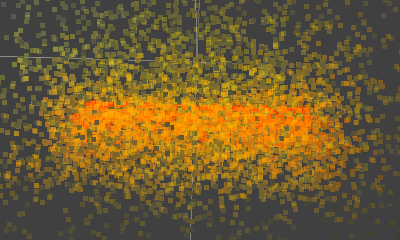
\includegraphics[width=25em]{img/transparency_no_back-to-front_ordering.png}
		\caption{Partikelsystem ohne Back-to-Front-Sortierung}
		\label{transparency-no-btf}
	\end{center}
\end{figure}
\textmd{\\Um die Transparenz korrekt darzustellen wurde eine Back-to-Front-Sortierung unter Zuhilfenahme der Binary-Space-Partition berechnet. Bei der Binary-Space-Partition werden die Partikel r�umlich durch Hyperebenen in einer Baumstruktur getrennt \cite[Folie 26]{jenke2016}. Jeder Partikel befindet sich dann entweder vor oder hinter einer Hyperebene, bei der er einsortiert wurde. Betrachtet man nun einen Sichtpunkt, so kann anhand der Hyperebenen die Back-to-Front-Sortierung ermittelt werden \cite[Folie 32]{jenke2016}.}
\textmd{\\Die Back-to-Front-Sortierung wiederum ist wichtig um die Partikel in der richtigen Reihenfolge zu zeichnen, sodass OpenGL die Transparenz korrekt darstellt. In der Darstellung des Beispiels aus Abbildung \ref{transparency-no-btf} mit Back-to-Front-Sortierung (siehe Abbildung \ref{transparency-with-btf}) fallen nun keine dunklen Partikel mehr auf. }
\begin{figure}[h]
	\begin{center}
		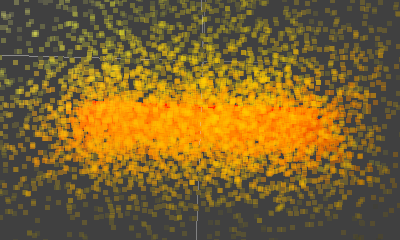
\includegraphics[width=25em]{img/transparency_with_back-to-front_ordering.png}
		\caption{Partikelsystem mit Back-to-Front-Sortierung}
		\label{transparency-with-btf}
	\end{center}
\end{figure}
